\documentclass{article}

\usepackage[english]{babel}

\usepackage[letterpaper,top=2cm,bottom=2cm,left=3cm,right=3cm,marginparwidth=1.75cm]{geometry}

\usepackage{amsmath}
\usepackage[section]{placeins}
\usepackage{graphicx}
\usepackage[colorlinks=true, allcolors=blue]{hyperref}

\usepackage{subfig}

\title{MIPS DATA SHEET - Team 3\vspace{-2em}}
\date{}

\setlength{\arrayrulewidth}{0.5mm}
\setlength{\tabcolsep}{30pt}
\renewcommand{\arraystretch}{1.5}

\begin{document}
\maketitle

\section{CPU Architecture Overview}

\begin{figure}[htp]
\centering
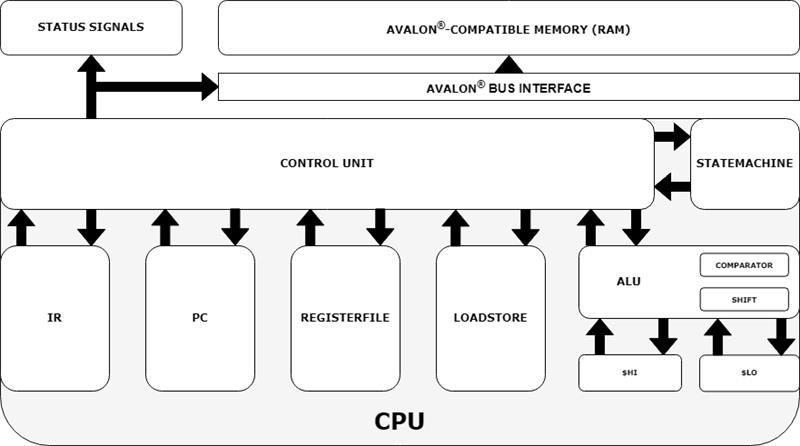
\includegraphics[width=0.7\textwidth]{top-level.jpg}
\end{figure}

\begin{tabular}[htp]{ |p{3cm}|p{8cm}|}
\hline
\multicolumn{2}{|c|}{Block Descriptions} \\
\hline
MIPS CPU Bus & This block is the main interface between the RAM
and the rest of the CPU. It adheres to Avalon(R)
specifications.  \\
Control Unit & This block handles the timings of the CPU and trans-
fers data to and from the other blocks. This block 
is the only block to directly interface with the CPU 
bus. \\
State Machine & This block controls the state the CPU is 
in - this block also enables the ability to stall, halt, 
and reset the CPU.  \\
Instruction 

Register & This block is responsible for decoding the instruction
and sending information to the Control Unit about 
the current Instruction Word. \\
Program Counter & This block keeps track of the address in the RAM of 
which instruction is currently being executed; setting this to 0 causes the CPU to halt. \\
Arithmetic Logic 

Unit & This block is responsible for all the arithmetic capabilities of the CPU, as well as comparator operations required for conditional branches.  \\
Load and Store & This block allows writing to the RAM as well as storing data from the RAM into the registers.  \\
Register File & This block contains all 32 MIPS registers, and has the ability to read from two registers at any point as well as to write data to any one register.\\
\hline
\end{tabular}


\section{Designing the CPU}

\subsection{Specification}

\subsubsection{CPU Interface:} This CPU adheres to the Avalon(R) specification, a memory bus-based interface, in order to be compatible with industrial IP blocks. Instructions and data are fetched over the same interface, and the memory has variable latency. This means that the CPU must be able to stall and wait for data transfer when it is not available - this was done with the help of CPU stalls from the state machine and Control Unit.
\subsubsection{Reset Behaviour:} When high, the CPU is to set all registers to 0, including the PC - this means that the CPU will halt immediately during a reset, however this causes the PC to take on the value of the reset vector, allowing it to continue execution as usual.
\subsubsection{Halt Behaviour:} When the CPU detects an attempt to execute an instruction at address 0, the CPU will halt - this is a special state where the 'active' flag of the CPU is low, thus showing that it has completed execution. In this state, register\_v0 is outputted on the bus to allow easy testing. This behaviour is exploited in our test-cases; all instructions end on a 'jr \$0' instruction, which will cause the PC to become 0 and therefore halt.

\subsection{Design Decisions}
In order to avoid complications, we decided to break down the CPU into several different units, and produce a CPU with several different files and connections, each file specialised for particular purpose.
Each block was tested separately, to ensure they worked, before recombining them. These different blocks are outlined above in the CPU Architecture Overview section.

\subsubsection{Bus vs Harvard}
We decided to develop a bus interface over a Harvard interface from the beginning, as we were all familiar with this particular architecture and converting a Harvard architecture to a bus-based one would require more effort.

\subsubsection{Control Unit}
To avoid the issue of coordinating timings between all the blocks, we decided to offload this task to the Control Unit, which sends signals to each block when the currently-executing instruction requires it - this also has the effect of preventing conflicts with other blocks such as when trying to request data from a register file. This means that each block had special inputs and outputs which had to be taken into consideration when designing the Control Unit.

\subsubsection{Standard Execution Cycle}
To make the design process more familiar to us, we decided to use the standard 3-cycle execution cycle per instruction, FETCH, EXEC1 and EXEC2, with the ability to stall each of these states and a halt state. This 3-stage execution is only possible if all the arithmetic instructions could be done in a single cycle, which we determined to be true.

\section{Testing the CPU}

\subsection{Testing Approach}

The process of testing and subsequent design improvement was a core part of our MIPS CPU development. Our process consisted of two main stages of testing: Initial testing of the individual CPU blocks and testing of the MIPS instruction set on the compiled CPU. 

\subsection{Stage 1}

After each block of the CPU was initially developed, a corresponding Verilog test bench was created alongside it to confirm that the individual blocks were implemented correctly. This step was carried out so that simple errors were dealt with early in the design process, and did not need to be dealt with later once the whole CPU is tested. The whole CPU is then compiled together. An additional Verilog test bench must be used to test if the inputs and outputs are correct and evaluate whether it is ready to be fully tested in stage 2.


\subsection{Stage 2}

The instruction testing stage aims to test the effectiveness of the whole CPU in executing each instruction from the MIPS instruction set. Test cases for each instruction were manually written in assembly language and converted by a MIPS assembler into machine code. The CPU is compiled with the test cases loaded into its RAM. The simulated CPU output is then compared with a reference output to check if the instruction was executed correctly. If tests fail, adequate adjustments are made to the implementation as a debugging step and this complete testing process is recursively repeated for every test case. 

\subsection{Test cases}
Test cases are split into 4 stages of testing which will be carried out in a specific order. This is important for debugging as it helps to highlight which specific blocks may be liable for errors since similar instructions will rely on the same CPU blocks. Any errors in the earlier stage instructions are likely to lead to errors in latter stage testing so it is important to follow a structured order such as this. 

\subsection{Stages of Test Cases}

\subsubsection{0 - Fundamental Testing:}
Fundamental instructions, these are core to testing the other instructions which may be dependent on them and hence they are tested first.

\subsubsection{1 – Arithmetic Testing:}
Arithmetic instructions which use the ALU. Most of the remaining testcases are heavily dependent on some of these instructions (mainly ADDIU and ADDU) in their testing and require them to function.

\subsubsection{2 – Conditionals:}
Conditional or branch instructions are tested next as they are reliant on the arithmetic instructions to produce the required conditions.

\subsubsection{3 – Other Test Cases:}
Finally, the remaining test cases should be tested to make sure every instruction is working. These may be slightly more complex or are dependent on previously tested instructions.
\hfill \break
\hfill \break

\subsection{Test Flow Diagram}

\begin{figure} [!htb]
    \centering
    \subfloat[\centering Stage 1 Testing ]{{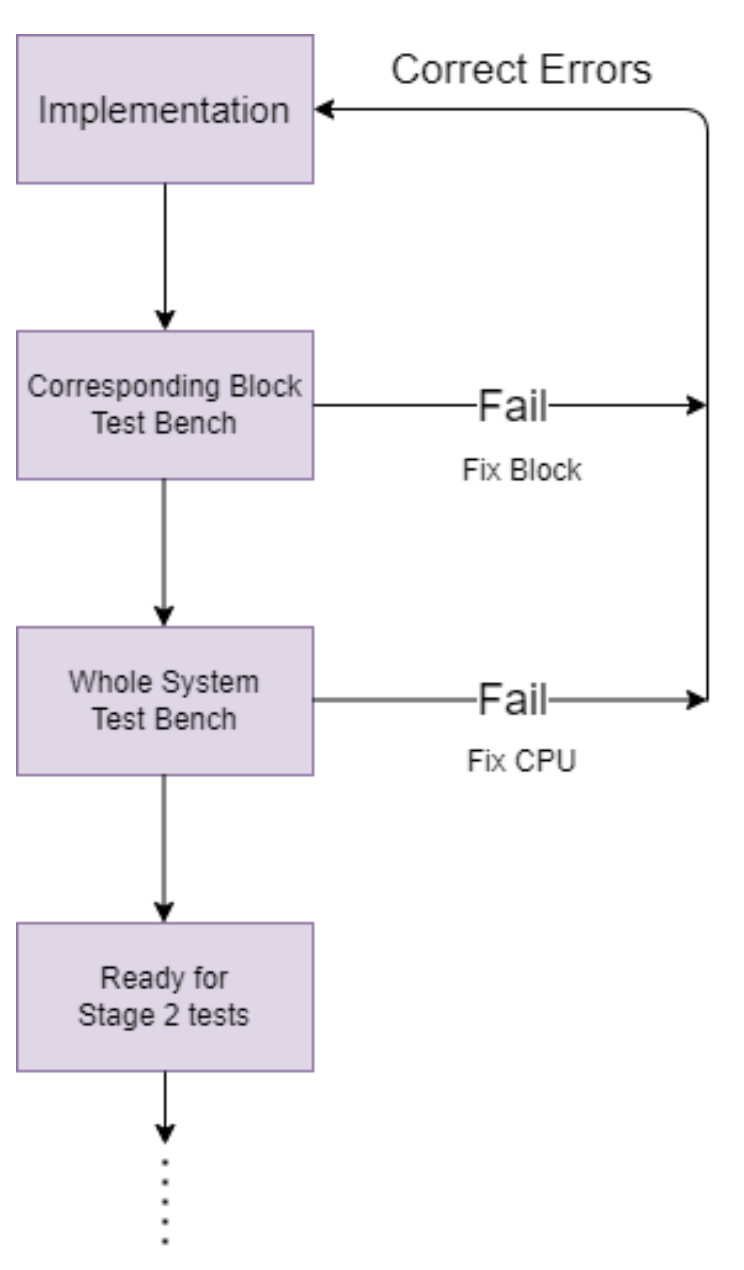
\includegraphics[width=3.5
cm]{testing1.png} }}%
    \qquad
    \subfloat[\centering Stage 2 Testing ]{{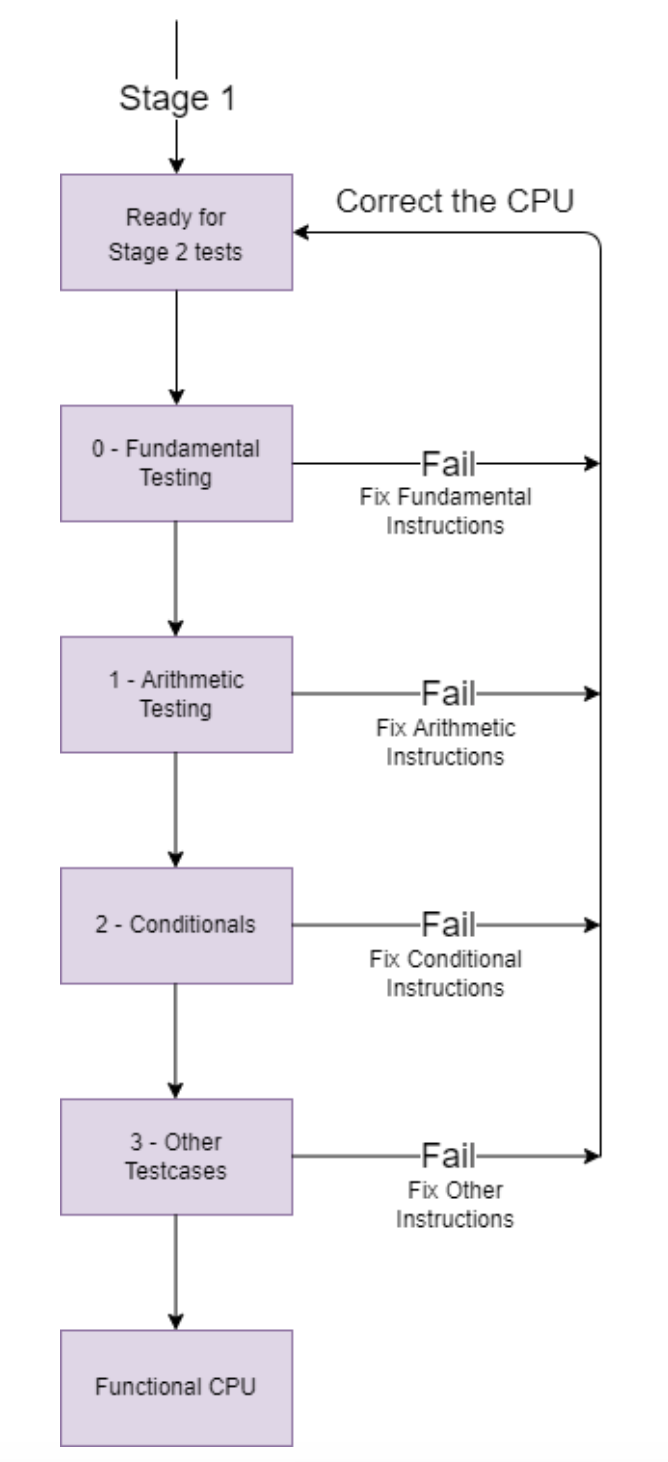
\includegraphics[width=3.5cm]{testing2.png} }}%

    \label{fig:example}%
\end{figure}


\section{Area and Timing Summary} 

A timing and area analysis, using Intel Quartus Prime, was run by configuring the CPU onto an Intel Cyclone IV FPGA. 

\hfill \break

\begin{tabular}[htp!]{ |p{5.95cm}|p{5.95cm}|}
\hline
\multicolumn{2}{|c|}{Area Summary} \\
\hline
Revision Name & \texttt{mips\_cpu\_bus}  \\
Top-Level Entity Name & \texttt{mips\_cpu\_bus} \\
Total Logic Elements Name & 6178/10,320 (60\%)  \\
Total Registers & 1036 \\
Total Pins & 138/180 (77\%) \\
Total Virtual Pins & 0  \\
Total Memory Bits & 0 / 423,936 (0\%) \\
Embedded Multiplier 9-bit elements & 8/46 (17\%)\\
Total PLLs & 0/2 (0\%)  \\
\hline
\end{tabular}

\hfill \break

\begin{tabular}{ |p{3cm}|p{3cm}|p{3cm}|  }
\hline
\multicolumn{3}{|c|}{Timing Summary} \\
\hline
FMax& Restricted FMax & Clock Name \\
\hline
143.04 MHz & 143.04 MHz & clk \\
\hline
\end{tabular}
\hfill \break
\hfill \break

\section{References}

Price, C., 1995,  \emph{MIPS IV Instruction Set} [Online]

Available at: \url{https://www.cs.cmu.edu/afs/cs/academic/class/15740-f97/public/doc/mips-isa.pdf} [Accessed 15 December 2021]

Soares, J., and Rocha, R., 2019-2020,  \emph{Encoding MIPS Instructions} [Online]

Available at: \url{https://www.dcc.fc.up.pt/~ricroc/aulas/1920/ac/apontamentos/P04_encoding_mips_instructions.pdf} [Accessed 16 December 2021]

OpenCores, 2019-2020,  \emph{Most MIPS I(TM) Opcodes} [Online]

Available at: \url{https://opencores.org/projects/plasma/opcodes} [Accessed 16 December 2021]

Berkeley, \emph{MIPS Reference Sheet} [Online]

Available at: \url{https://inst.eecs.berkeley.edu/~cs61c/resources/MIPS_help.html} [Accessed 17 December 2021]

Pakin, S., 2021, \emph{The Comprehensive LATEX Symbol List} [Online]

Available at: \url{http://tug.ctan.org/info/symbols/comprehensive/symbols-a4.pdf} [Accessed 17 December 2021]

\end{document}
